%
% entwicklungssatz.tex -- neue version der Darstelllung des Entwicklungssatzes
%
% (c) 2017 Prof Dr Andreas Müller, Hochschule Rapperswil
%
\subsection{Entwicklungsssatz aus der Pivotproduktformel}
Die Pivotproduktformel erlaubt, die Determinante einer Dreiecksmatrix sofort
zu berechnen:
\[
\left|\begin{matrix}
a_{11}&a_{12}&a_{13}&\dots &a_{1n}\\
  0   &a_{22}&a_{23}&\dots &a_{2n}\\
  0   &  0   &a_{33}&\dots &a_{3n}\\
\vdots&\vdots&\vdots&\ddots&\vdots\\
  0   &  0   &   0  &  0   &a_{nn}
\end{matrix}\right|
=
a_{11}\cdot a_{22}\cdot a_{33}\cdot\dots\cdot a_{nn}.
\]
Es lässt sich daraus aber eine viel allgemeinere Beobachtung ableiten, die
schliesslich zu einer allgemeinen Berechnungsformel für die Determinante
führt, dem Entwicklungssatz.

\subsubsection{Rekursion}
Wir betrachten die Determinante, die in der ersten Spalte nur in der
ersten Zeile ein von Null verschiedenes Element enthält:
\[
%\left|\begin{matrix}
A=
\begin{pmatrix}
a_{11}&a_{12}&a_{13}&\dots &a_{1n}\\
  0   &a_{22}&a_{23}&\dots &a_{2n}\\
  0   &a_{32}&a_{33}&\dots &a_{3n}\\
\vdots&\vdots&\vdots&\ddots&\vdots\\
  0   &a_{n2}&a_{n3}&\dots &a_{nn}
\end{pmatrix}.
%\end{matrix}\right|
\]
Nach der Pivotproduktformel ist $a_{11}$ das erste Pivot-Element.
Es muss jetzt nur noch der Gaussalgorithmus in der verbleibenden Matrix
\[
A_{11}
=
\begin{pmatrix}
a_{22}&a_{23}&\dots &a_{2n}\\
a_{32}&a_{33}&\dots &a_{3n}\\
\vdots&\vdots&\ddots&\vdots\\
a_{n2}&a_{n3}&\dots &a_{nn}
\end{pmatrix}
\]
bestimmt werden.
Die weggelassene erste Zeile und Spalte hat keinen Einfluss darauf, wie
der Gauss-Algorithmus in $A_{11}$ durchgeführt wird.
Die Pivotproduktformel liefert daher die Rekursionsformel
\begin{equation}
\det(A)
=
a_{11}\cdot
\left|\begin{matrix}
a_{22}&a_{23}&\dots &a_{2n}\\
a_{32}&a_{33}&\dots &a_{3n}\\
\vdots&\vdots&\ddots&\vdots\\
a_{n2}&a_{n3}&\dots &a_{nn}
\end{matrix} \right|
=
a_{11}
\det(A_{11}).
\label{determinante:entwicklungssatz:rekursion}
\end{equation}

\subsubsection{Vorzeichenregel}
Die Rekursionsformel~\eqref{determinante:entwicklungssatz:rekursion}
kann verallgemeinert werden auf eine Situation, wo in Spalte $k$
nur ein Element, nämlich das in Zeile $i$, von Null verschieden ist.
\[
A=
\begin{pmatrix}
a_{  1 1}&\dots &a_{  1,k-1}&a_{  1 k}&a_{  1,k+1}&\dots &a_{  1 n}\\
\vdots   &\ddots&\vdots     &\vdots   &\vdots     &\ddots&\vdots   \\
a_{i-1,1}&\dots &a_{i-1,k-1}&a_{i-1,k}&a_{i-1,k+1}&\dots &a_{i-1,n}\\
a_{  i 1}&\dots &a_{  i,k-1}&a_{  i k}&a_{  i,k+1}&\dots &a_{  i n}\\
a_{i+1,1}&\dots &a_{i+1,k-1}&a_{i+1,k}&a_{i+1,k+1}&\dots &a_{i+1,n}\\
\vdots   &\ddots&\vdots     &\vdots   &\vdots     &\ddots&\vdots   \\
a_{  n 1}&\dots &a_{  n,k-1}&a_{  n k}&a_{  n,k+1}&\dots &a_{  n n}
\end{pmatrix}
\]
Durch Vertauschung mit den $i-1$ vorangegangenen Zeilen und $k-1$
vorangegangen Spalten kann man erreichen, dass das Element $a_{ik}$
in die linke obere Ecke verschoben wird.
Bei den Zeilenvertauschungen ändert das Vorzeichen $(i-1)$-mal, also
um $(-1)^{i-1}$, bei den Spaltenvertauschungen um den Faktor $(-1)^{k-1}$.
Insgesamt erhalten wir daher die Formel
\begin{align*}
\det(A)
&=
(-1)^{i-1}(-1)^{k-1}
\left|\;\begin{matrix}
a_{ik}&a_{  i 1}&\dots &a_{  i,k-1}&a_{  i,k+1}&\dots &a_{  i n}\\
  0   &a_{  1 1}&\dots &a_{  1,k-1}&a_{  1,k+1}&\dots &a_{  1 n}\\
\vdots&\vdots   &\ddots&\vdots     &\vdots     &\ddots&\vdots   \\
  0   &a_{i-i,1}&\dots &a_{i-i,k-1}&a_{i-1,k+1}&\dots &a_{i-i,n}\\
  0   &a_{i+i,1}&\dots &a_{i+i,k-1}&a_{i+1,k+1}&\dots &a_{i+i,n}\\
\vdots&\vdots   &\ddots&\vdots     &\vdots     &\ddots&\vdots   \\
  0   &a_{  n 1}&\dots &a_{  n,k-1}&a_{  n,k+1}&\dots &a_{  n n}
\end{matrix}\;\right|
\\
&=
(-1)^{i+k-2}
\cdot
a_{ik}
\cdot
\left|\;\begin{matrix}
a_{  1 1}&\dots &a_{  1,k-1}&a_{  1,k+1}&\dots &a_{  1 n}\\
\vdots   &\ddots&\vdots     &\vdots     &\ddots&\vdots   \\
a_{i-i,1}&\dots &a_{i-i,k-1}&a_{i-1,k+1}&\dots &a_{i-i,n}\\
a_{i+i,1}&\dots &a_{i+i,k-1}&a_{i+1,k+1}&\dots &a_{i+i,n}\\
\vdots   &\ddots&\vdots     &\vdots     &\ddots&\vdots   \\
a_{  n 1}&\dots &a_{  n,k-1}&a_{  n,k+1}&\dots &a_{  n n}
\end{matrix}\;\right|
=
(-1)^{i+k}\det(A_{ik}),
\end{align*}
darin haben wir mit $A_{ik}$ die Matrix abgekürzt, die aus $A$ durch
Weglassen der Zeile $i$ und der Spalte $k$ entsteht.
Das Vorzeichen $(-1)^{i+k}$ kann dem folgenden Schachbrettmuster
entnommen werden:
\begin{center}
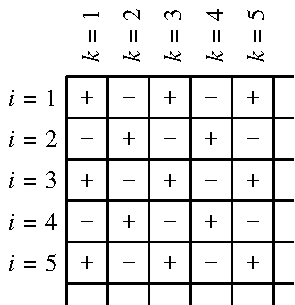
\includegraphics{2/images/schachbrett.pdf}
\end{center}

\subsubsection{Aufteilung einer Spalte}
Enthält eine Spalte nur ein einziges von Null verschiedenes Element,
können wir die Determinante auf die Berechnung einer kleineren
Determinante reduzieren.
Um dies für die Berechnung einer beliebigen Determinante ausnützen
zu können, müssen wir in der Lage sein, eine beliebige Spalte in Spalten
aufzuteilen, die nur ein einziges von Null verschiedenes Element
enthalten.
Dies gelingt mit Hilfe der Linearität.

Wir zeigen das Prinzip am Beispiel der ersten Spalte.
Die Linearität liefert
\begin{align}
\left|\begin{array}{cccc}
a_{11}&a_{12}&\dots &a_{1n}\\
a_{21}&a_{22}&\dots &a_{2n}\\
a_{31}&a_{32}&\dots &a_{3n}\\
\vdots&\ddots&\ddots&\vdots\\
a_{n1}&a_{n2}&\dots &a_{nn}\\
\end{array}\right|
&=
\left|\begin{array}{c@{\hskip2pt}c@{\hskip2pt}cccc}
a_{11}&+&  0   &a_{12}&\dots &a_{1n}\\
  0   &+&a_{21}&a_{22}&\dots &a_{2n}\\
  0   &+&a_{31}&a_{32}&\dots &a_{3n}\\
\vdots& &\vdots&\ddots&\ddots&\vdots\\
  0   &+&a_{n1}&a_{n2}&\dots &a_{nn}\\
\end{array}\right|
\notag
\\
&=
\left|\begin{array}{cccc}
a_{11}&a_{12}&\dots &a_{1n}\\
  0   &a_{22}&\dots &a_{2n}\\
  0   &a_{32}&\dots &a_{3n}\\
\vdots&\ddots&\ddots&\vdots\\
  0   &a_{n2}&\dots &a_{nn}\\
\end{array}\right|
+
\left|\begin{array}{cccc}
  0   &a_{12}&\dots &a_{1n}\\
a_{21}&a_{22}&\dots &a_{2n}\\
a_{31}&a_{32}&\dots &a_{3n}\\
\vdots&\ddots&\ddots&\vdots\\
a_{n1}&a_{n2}&\dots &a_{nn}\\
\end{array}\right|.
\label{determinate:entwicklungssatz:aufspaltung}
\end{align}
Durch wiederholte Anwendung dieser Idee kann die erste Spalte in $n$
Spalten aufgeteilt werden, die jede nur ein einziges von Null verschiedenes
Element enthält.

\subsubsection{Allgemeiner Fall}
Damit haben wir alle Komponenten für die allgemeine Berechnungsformel
zusammen.
Wir wählen dazu die Spalte $k$ aus.
Die Aufspaltungsformel
\eqref{determinate:entwicklungssatz:aufspaltung}
besagt, dass wir eine Determinante zerlegen können in eine Summe von
speziellen Determinanten, in denen die Spalte $k$ jeweils nur ein
von Null verschiedenes Elemente enthält.
Diese Elemente sind die Spaltenelemente $a_{ik}$ mit $1\le i\le n$.

Die Rekursionsformel \eqref{determinante:entwicklungssatz:rekursion}
besagt, dass wir diese Determinanten berechnen können aus der
Determinante der Matrix, in der man die Zeile $i$ und die Spalte $k$
weggelassen hat.
Die Vorzeichenregel sagt, welches Vorzeichen man dazu verwenden muss.
Insgesamt bekommen wir so die Formel
\[
\det(A)
=
\sum_{i=1}^n
\underbrace{ (-1)^{i+k}}_{\text{Vorzeichen }}
\underbrace{
a_{ik}
\cdot
\det(A_{ik}).
}_{\text{Rekursion nach 
\eqref{determinante:entwicklungssatz:rekursion}}}
\]
Sie heisst der {\em Entwicklungssatz}.
\index{Entwicklungssatz}


